As already described in the subchapters \ref{subchap:nature} and \ref{subchap:reinterpreting}, it is also possible to express the overall task as an imitation problem, where the agent directly tries to mimic the underlying policy of a human expert—the captain. In the case of behavioral cloning, the agent does not explore the state space nor receives rewards anymore, but instead learns the state and action distributions in a supervised manner. Here, the dataset consists of simplified transition tuples of just $(s_t, a_t)$ where the features of $s_t$ are the input to the policy network and $a_t$ marks the desired output. The dataset is generated by recording the current state of the GT, as well as the next heading and speed values as expert action, based on the presented functions that produce $curve\_A$, $curve\_B$ and $curve\_C$, i.e., Eq. \ref{eq:curve_A}.
\par
When exposing behavioral cloning to the same task of generating trajectories that are identically to the GT curves, it shows better performance in contrast to DDPG throughout all experiment setups. This is indeed an expected outcome, as a big enough neuronal network should be able to overfit to the training data and thus learn the perfect mapping of states to actions. Nevertheless, different network architectures show deviating performances, which suggests the need for further investigations. In this context, we conduct a series of experiments, testing different learning rates and network settings. The results for all these experiments can be found in the appendix in section \ref{appendix:curveResults}.
\par
We found out that the default network architecture of the used library \textit{imitation} of $n_{h}^{1}=100$ and $n_{h}^{2}=100$ can be improved, not only by the raw amount of neurons in each hidden layer, but also by the proportion of the different hidden layers. Generally, we notice that having consecutive hidden layers with reducing amounts of neurons yield better results than an equal proportion regardless of the number of neurons. For the real-world applicable state representation $S3$, the best outcome is achieved by a fully-connected neuronal network comprised of $n_{h}^{1}=256, n_{h}^{2}=128$ and $n_{h}^{3}=64$, which is trained for 15k epochs with a learning rate of $\alpha = 10^{-5}$. The upcoming Figs. \ref{fig:bcCurves1} and \ref{fig:bcCurves2} visualize the behavior of the trained policy network that has a performance of $2.92 \pm 2.28$. Please note, that the y limits of the graph in Fig. \ref{fig:bcCurves1} are different from the graphs of the previous chapter.

\begin{figure}[H]
     \centering
         \includesvg[width=0.9\textwidth]{images/bc_curve_results/bc_S3_A2_256_128_64_5lr.svg}
        \caption{Performance of behavioral cloning over time during the three different episodes. Learning rate $\alpha = 10^{-5}$ trained for 15k epochs with a network architecture of $n_{h}^{1}=256, n_{h}^{2}=128$ and $n_{h}^{3}=64$.}
        \label{fig:bcCurves1}
\end{figure}


\begin{figure}[H]
     \centering
     \begin{subfigure}[b]{0.31\textwidth}
         \centering
         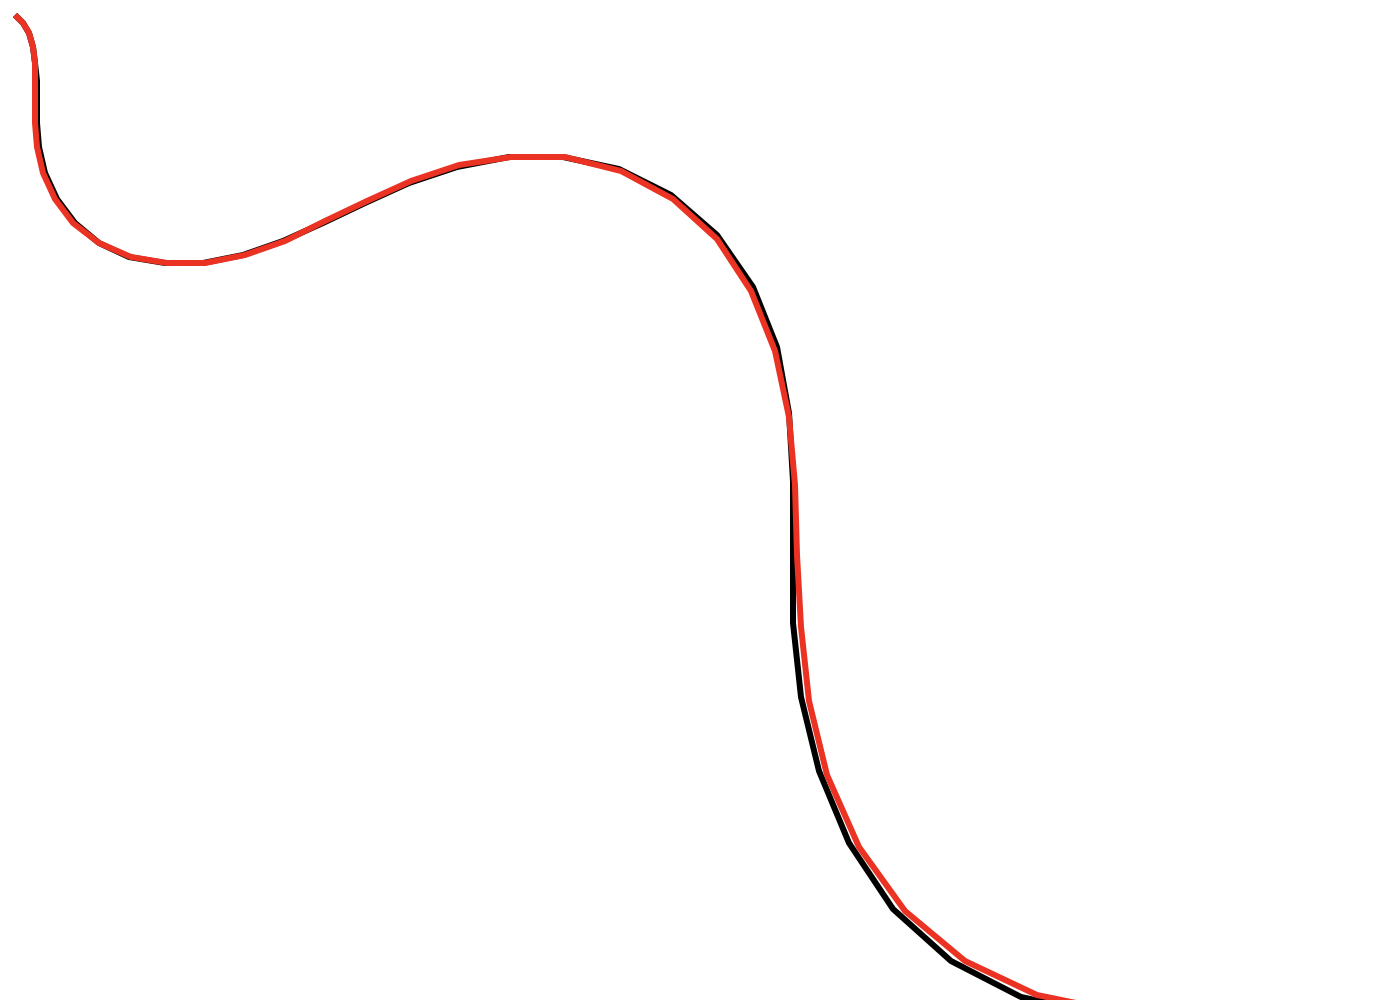
\includegraphics[width=\textwidth]{images/bc_curve_results/S3_A2_256_128_64_curve_A.png}
         \caption{$curve\_A$}
     \end{subfigure}
     \hfill
     \begin{subfigure}[b]{0.31\textwidth}
         \centering
         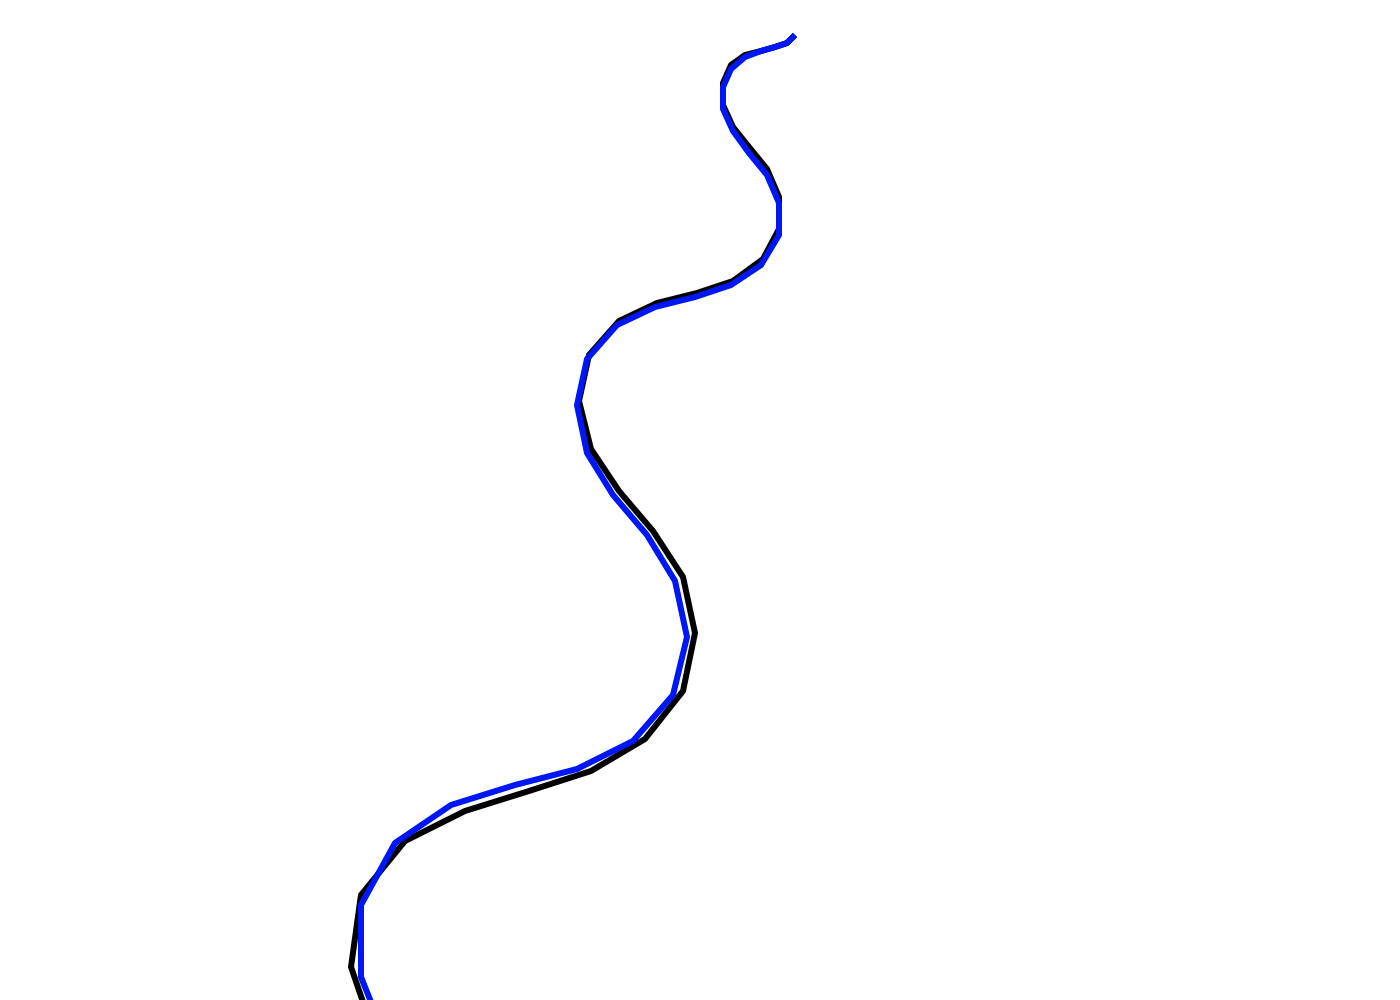
\includegraphics[width=\textwidth]{images/bc_curve_results/S3_A2_256_128_64_curve_B.png}
         \caption{$curve\_B$}
     \end{subfigure}
     \hfill
     \begin{subfigure}[b]{0.31\textwidth}
         \centering
         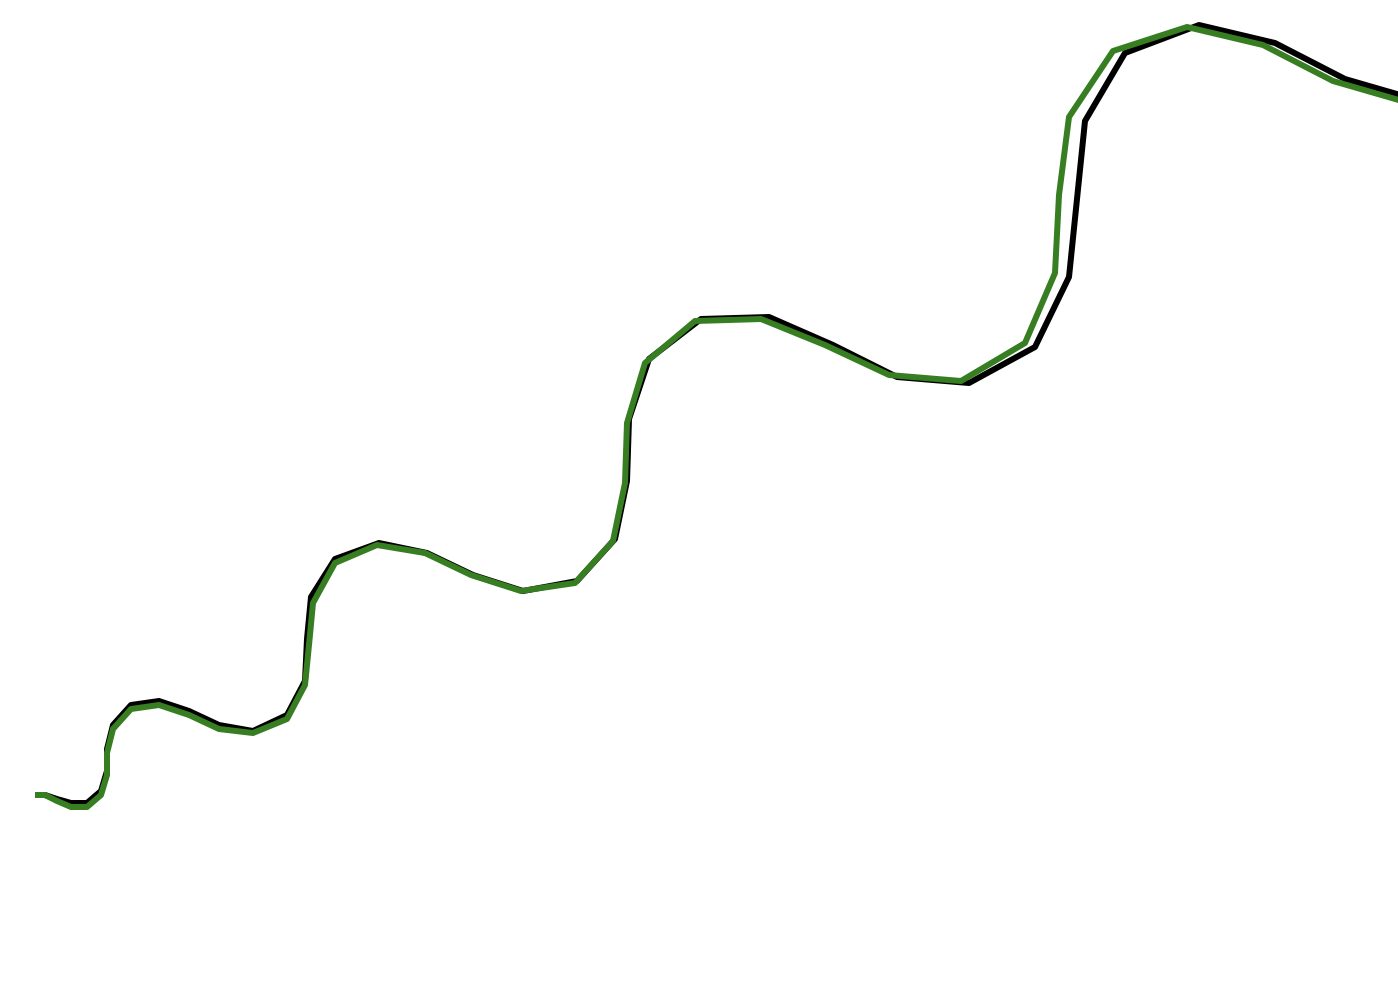
\includegraphics[width=\textwidth]{images/bc_curve_results/S3_A2_256_128_64_curve_C.png}
         \caption{$curve\_C$}
     \end{subfigure}
        \caption{$S3\_A2$, learning rate $\alpha = 10^{-5}$ trained for 15k epochs with a network architecture of $n_{h}^{1}=256, n_{h}^{2}=128$ and $n_{h}^{3}=64$.}
        \label{fig:bcCurves2}
\end{figure}

